\documentclass[xcolor=x11names,compress]{beamer}
\usepackage[english]{babel}

%% General document %%%%%%%%%%%%%%%%%%%%%%%%%%%%%%%%%%
\usepackage{graphicx}
\usepackage{tikz}
\usepackage{wrapfig}
\usepackage{hyperref}
\usepackage{fancybox}
\usetikzlibrary{arrows}
\tikzstyle{block}=[draw opacity=0.7,line width=1.4cm]
\usetikzlibrary{decorations.fractals}
%%%%%%%%%%%%%%%%%%%%%%%%%%%%%%%%%%%%%%%%%%%%%%%%%%%%%%


%% Beamer Layout %%%%%%%%%%%%%%%%%%%%%%%%%%%%%%%%%%
\useoutertheme[subsection=false,shadow]{miniframes}
\useinnertheme{default}
\usefonttheme{serif}
\usepackage{palatino}

\setbeamerfont{title like}{shape=\scshape}
\setbeamerfont{frametitle}{shape=\scshape}

\setbeamercolor*{lower separation line head}{bg=DeepSkyBlue4} 
\setbeamercolor*{normal text}{fg=black,bg=white} 
\setbeamercolor*{alerted text}{fg=red} 
\setbeamercolor*{example text}{fg=black} 
\setbeamercolor*{structure}{fg=black} 
 
\setbeamercolor*{palette tertiary}{fg=black,bg=black!10} 
\setbeamercolor*{palette quaternary}{fg=black,bg=black!10} 


\newenvironment<>{problock}[1]{%
  \begin{actionenv}#2%
      \def\insertblocktitle{#1}%
      \par%
      \mode<presentation>{%
        \setbeamercolor{block title}{fg=white,bg=DeepSkyBlue4}
       \setbeamercolor{block body}{fg=black,bg=black!10}
       \setbeamercolor{itemize item}{fg=blue!20!black}
       \setbeamertemplate{itemize item}[triangle]
     }%
      \usebeamertemplate{block begin}}
    {\par\usebeamertemplate{block end}\end{actionenv}}


\useinnertheme[shadow=true]{rounded}


\renewcommand{\(}{\begin{columns}}
\renewcommand{\)}{\end{columns}}
\newcommand{\<}[1]{\begin{column}{#1}}
\renewcommand{\>}{\end{column}}
%%%%%%%%%%%%%%%%%%%%%%%%%%%%%%%%%%%%%%%%%%%%%%%%%%
\newcommand{\hlb}[1]{\textbf{\textcolor{blue}{#1}}}
\newcommand{\hl}[1]{\textcolor{blue}{#1}}
\newcommand{\lien}[2]{\mathcal{L}_{#1}^{#2}}
\newcommand{\lie}[1]{\mathcal{L}_{#1}}

\newcommand{\colv}[2]{\begin{pmatrix}#1\\#2\end{pmatrix}}

%\usepackage[english]{babel}
\usepackage[utf8]{inputenc}
%\usetheme{Goettingen}

\begin{document}
\title{Bifurcations in continuous time dynamical systems}
\author{Debsankha Manik}

\begin{frame}
\titlepage
\end{frame}

\begin{frame}{Fixed points by Newton-Raphson Method}
After grazing, a new period-1 orbit gains stability (sometimes after a short 
spell of chaos) 


\begin{figure}
\begin{center}
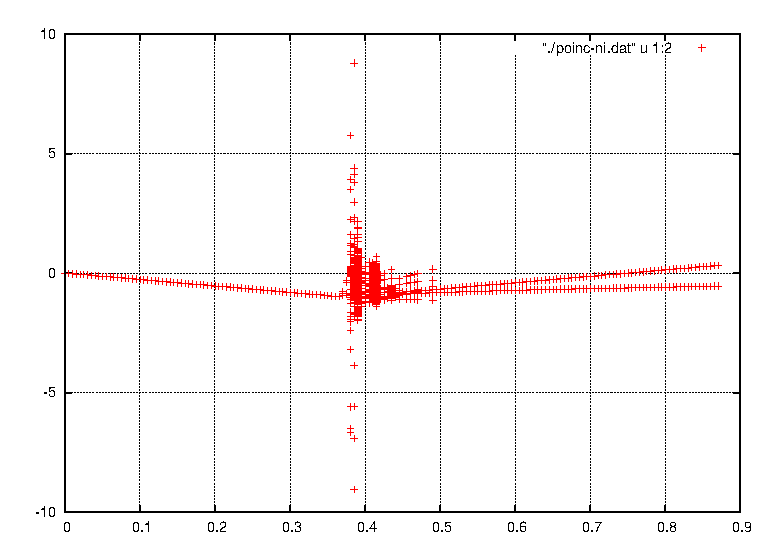
\includegraphics[width=0.9\columnwidth]{after-graz-non-int}
\end{center}
\end{figure}
\end{frame}

\begin{frame}
\begin{figure}
\begin{center}
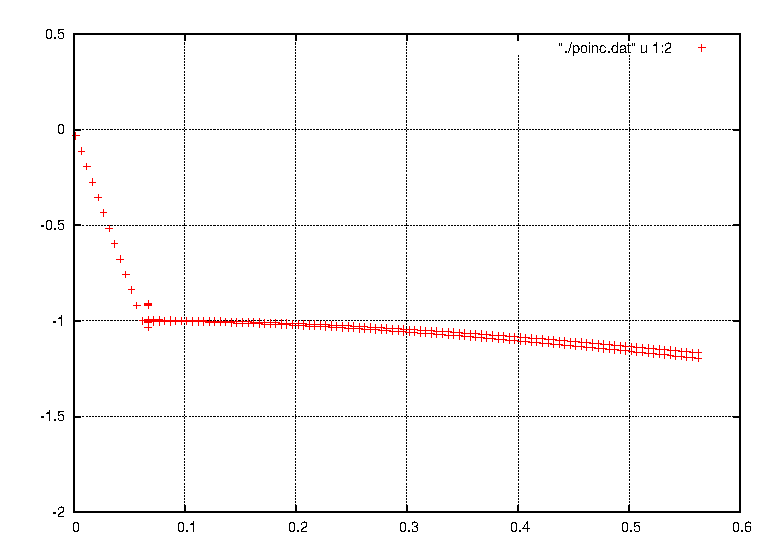
\includegraphics[width=0.9\columnwidth]{after-graz-int}
\end{center}
\end{figure}
\end{frame}

\begin{frame}
\begin{figure}
\caption{}
\begin{center}
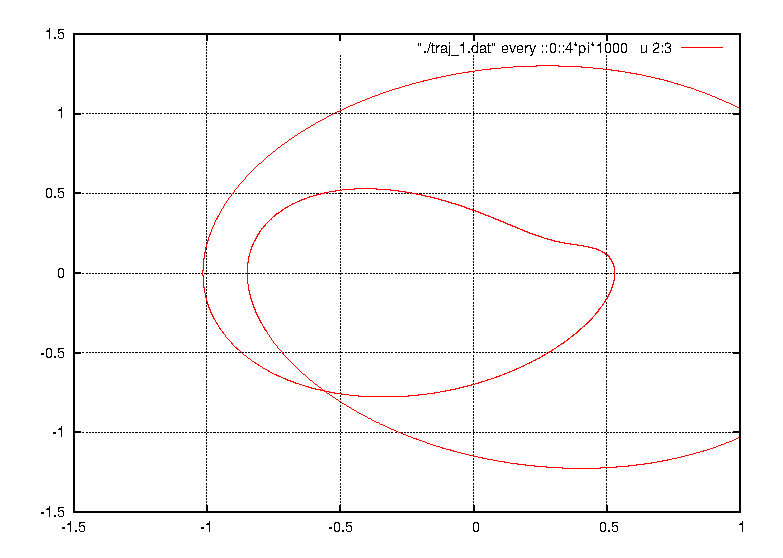
\includegraphics[width=0.9\columnwidth]{after-grazing-p1-traj}
\end{center}
\end{figure}
\end{frame}

\begin{frame}{How to pinpoint  these fixed points?}
Define a 5-dim vector $y=(x_0,v_0,x_c,v_c,\tau)$.  \\
And a system of equations:
\begin{align*}
G_{1,2}(y)=\vec{x_1}-\varphi(\tau,0,\vec{x_0})&=0\\
G_{3,4}(y)=\vec{x_0}-\varphi(2T,\tau,\vec{x_1})&=0\\
G_5(y)=x_1-\sigma&=0
\end{align*}

Then we can solve the equation $G(y)=0$ using NR method:
\[
y_{n+1}=y_n+J(y)^{-1}G(y)
\]
\end{frame}

\begin{frame}
\begin{figure}
\caption{Eigenvalues of the fixed points vs.   bifurcation parameter}
\begin{center}
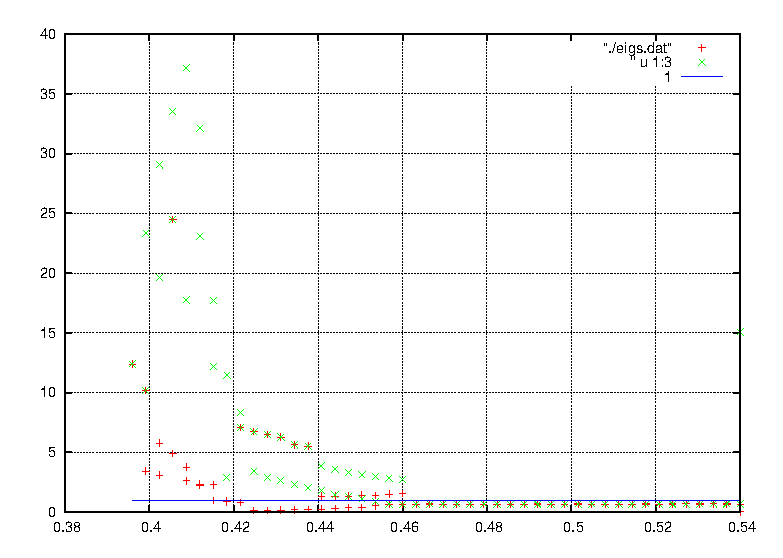
\includegraphics[width=0.9\columnwidth]{eigvals}
\end{center}
\end{figure}
\end{frame}

\begin{frame}{Problems}
\begin{itemize}
\item Sometimes we get unphysical fixed points.  \\
\item We get 2 fixed points for each period-1 orbit\\
\item Sometimes, the eigenvalues of those 2 fixed points are different!
\end{itemize}
\end{frame}


\begin{frame}{Impact map approach}
C.   Budd, F.   Dux, A.   Cliffe, The effect of frequency and clearance 
variations on single-degree-of-freedom impact oscillators, Journal of Sound 
and Vibration, Volume 184, Issue 3, 20 July 1995
\begin{figure}
\caption{Impact map in case of $PnC1$ orbit}
\begin{center}
\includegraphics[width=0.5\columnwidth]{impactmap}
\end{center}
\end{figure}
\end{frame}

\begin{frame}{Derivation}
Budd et al did it for the without damping. Introduction of damping makes 
things more interesting, as we will see.  \\
\begin{align}
\colv{x^-(\tau)}{v^-(\tau)}&=\colv{x_p(\tau)}{v_p(\tau)}+\colv{x_h(\tau)}{v_h(\tau)}\\
\colv{x^+(\tau)}{v^+(\tau)}&=\colv{x_p(\tau)}{v_p(\tau)}+\colv{x_h(\tau)}{-v_h(\tau)-2v_p(\tau)}\\
\colv{x^-(\tau+nT)}{v^-(\tau+nT)}&=\colv{x_p(\tau+nT)}{v_p(\tau+nT)}+M(nT)\colv{x_h(\tau)}{-v_h(\tau)-2v_p(\tau)}\\
&=\colv{x_p(\tau)}{v_p(\tau)}+M(nT)\colv{x_h(\tau)}{-v_h(\tau)-2v_p(\tau)}
\end{align}
\end{frame}

\begin{frame}
Provided a $PnC1$ orbit exists (stable or unstable),
\[
M(nT)\colv{x_h(\tau)}{-v_h(\tau)-2v_p(\tau)}=\colv{x_h(\tau)}{v_h(\tau)}
\]

and 
\[
x_p(\tau)+x_h(\tau)=\sigma
\]

We recall:
\[
x_p(t)=A\footnote{$A=F/\sqrt{(\omega_0^2-\omega^2)^2+\omega^2\gamma^2}$}cos(\omega t+tan^{-1}\frac{\omega \gamma}{\omega^2-\omega_0^2})
\]

\begin{align*}
v_p(t)&=-A\omega sin(\omega t+tan^{-1}\frac{\omega \gamma}{\omega^2-\omega_0^2})\\
&=\mp A\omega \sqrt{1-\left(\frac{x_p}{A}\right)^2}\\
&=\mp A\omega \sqrt{1-\left(\frac{\sigma-x_h}{A}\right)^2}
\end{align*}

\end{frame}
\begin{frame}
The condition for existence of a $PnC1$ orbit:
\begin{equation}
\label{impactmap-final}
M(nT)\colv{x}{-v\pm2\omega \sqrt{A^2-(\sigma-x_h})^2}=\colv{x}{v}
\end{equation}

The uncertainty about the $\pm$  sign is slightly unsettling.  There actually 
\emph{isn't} any justification for choosing one sign over the other : it is a 
direct consequence of the fact that for the same position, the velocity of the 
oscillator can have two values equal in magnitude but with opposite signs.  

Suppose
\[
M(nT)=
\begin{pmatrix}
a & b\\
c & d
\end{pmatrix}
\]

\end{frame}
\begin{frame}{Equations for the fixed point}
\begin{align}
\label{fp-separate}
x&=ax-bv \pm 2b\omega\sqrt{A^2-(\sigma-x)^2}\\
v&=cx-dv \pm 2d\omega\sqrt{A^2-(\sigma-x)^2}
\end{align}

$v$ can be easily eliminated:
\begin{align*}
\frac{x(1-a)+bv}{b}&=\frac{v(1+d)-cx}{d}\\
bv&=x(d-ad+bc)
\end{align*}

Substituting in \eqref{fp-separate}:
\begin{align*}
x(a-d+ad-bc-1)\pm 2b\omega\sqrt{A^2-(\sigma-x)^2}&=x\\
A^2-(\sigma-x)^2-\left\{\frac{(a-d+ad-bc-1)}{2b\omega}\right\}^2x^2&=0
\end{align*}
\end{frame}


\begin{frame}
Let \[
\alpha=\frac{(a-d+ad-bc-1)}{2b\omega}
\]

Then:
\begin{align*}
A^2-(\sigma-x)^2&=\alpha^2x^2\\
x^2(\alpha^2+1)-2\sigma x+(\sigma^2-A^2)&=0
\end{align*}

Therefore we have the solution:
\begin{align}
\label{fp-solution}
x^*&=\frac{\sigma\pm\sqrt{\sigma^2-(\alpha^2+1)(\sigma^2-A^2)}}{\alpha^2+1}\\
v^*&=\frac{(d-ad+bc)x^*}{b}
\end{align}

\end{frame}




\end{document}
